\documentclass[11pt]{article}

\usepackage[margin=1in]{geometry}
\usepackage{amsmath,amssymb,amsfonts,bm}
\usepackage{graphicx}
\usepackage{xcolor}
\usepackage{float}
\usepackage{listings}
\usepackage{enumitem}
\usepackage{booktabs}
\usepackage{hyperref}
\usepackage{xurl}
\usepackage{fancyhdr}

% ---------- URL and Hyperlink setup ----------
\Urlmuskip=0mu plus 1mu
\hypersetup{
	breaklinks=true,
	colorlinks=true,
	linkcolor=blue,
	urlcolor=blue
}

% ---------- Code style ----------
\lstdefinestyle{matlabstyle}{
	language=Python,
	basicstyle=\ttfamily\small,
	numbers=left,
	numberstyle=\tiny,
	stepnumber=1,
	numbersep=8pt,
	frame=single,
	columns=fullflexible,
	keepspaces=true,
	showstringspaces=false,
	keywordstyle=\bfseries,
	commentstyle=\itshape\color{gray},
}

% ---------- Header setup ----------
\pagestyle{fancy}
\fancyhf{}
\fancyhead[L]{November 2, 2025}
\fancyhead[C]{ECE 517: Homework 3.2}
\fancyhead[R]{Scott Nguyen}
\renewcommand{\headrulewidth}{0.4pt}
\fancyfoot[C]{\thepage}

\begin{document}
	
	\begin{enumerate}
		\item Copy and run the following code to construct some toy data
		
		\vspace{0.5em}
		\noindent\textbf{Solution.}
		
		\begin{figure}[H]
			\centering
			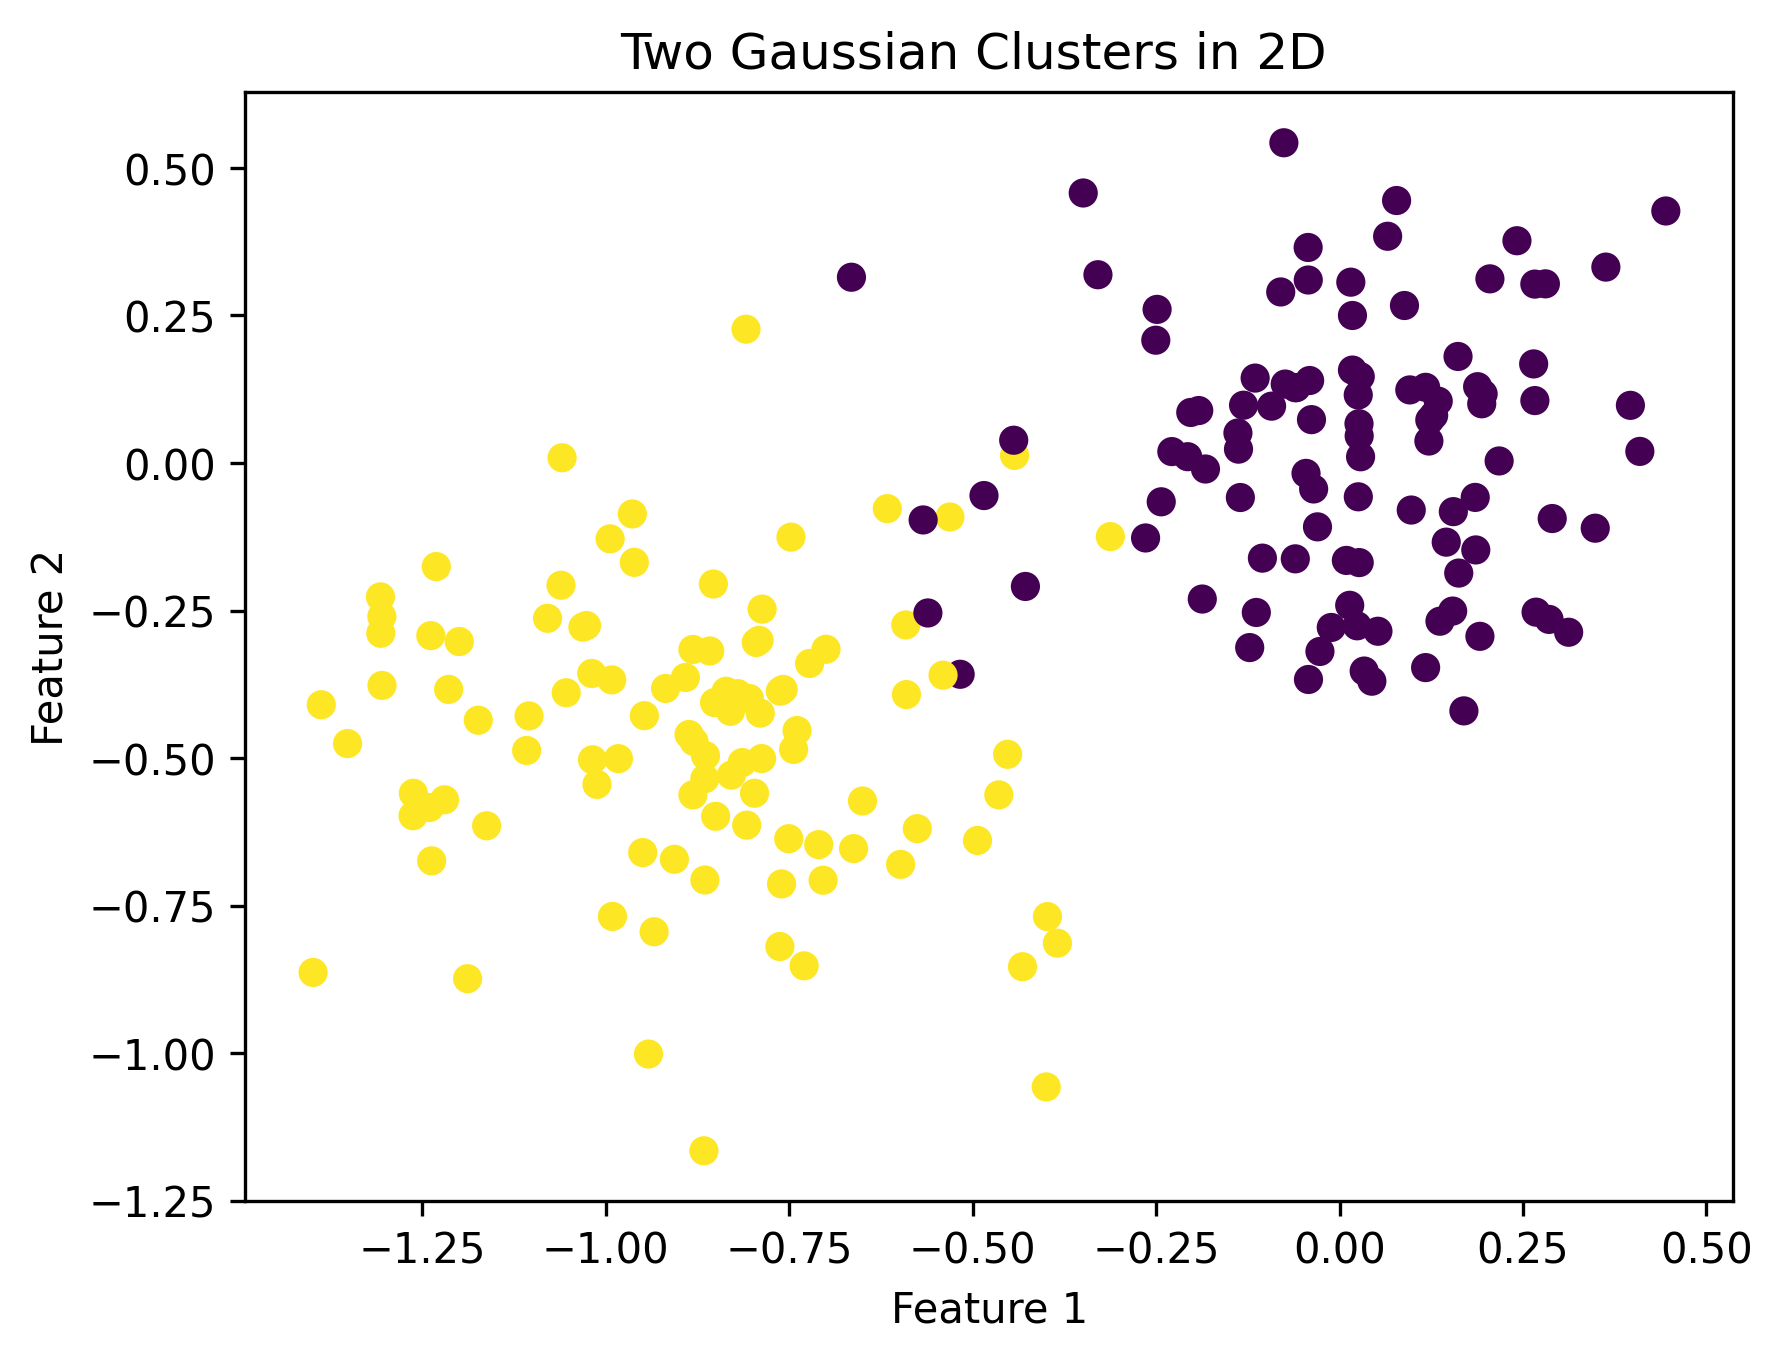
\includegraphics[width=0.55\textwidth]{Code/plots/p1.png}
			\caption{Two Gaussian clusters in 2D with labels $-1$ and $+1$.}
		\end{figure}
		
		\item The code below is an example of a SVM classifier. By using it, write a code that trains a linear SVM for classification. Represent in the same graph the classification boundary, the margins and the support vectors. 
		\vspace{0.5em}
		
		\noindent\textbf{Solution.}
		
		\begin{figure}[H]
			\centering
			
\includegraphics[width=0.55\textwidth]{code/plots/p2.png}
			\caption{Linear SVM classification boundary, margins, and support vectors.}
		\end{figure}
		
		\newpage
		
		\item The following code generates a set of clusters $(N_{\text{clusters}})$ in a space of $N_{\text{dim}}$ dimensions. Each cluster contains data with labels $+1$ or $-1$. The number of dimensions must be at least equal to the number of clusters minus one for the data to be linearly separable.
		
		\medskip
		\noindent\textbf{3.1} Find the value of $C$ that produces the best validation error. Repeat the experiment 100 times with different training and validation data and average the values of the optimal $C$ ($C_{\text{opt}}$) and the corresponding averaged error ($E_{\text{opt}}$). The error must be defined as the fraction of misclassified samples (not MSE). 
		
		Perform the experiment for the following configurations:
		\begin{itemize}
			\item 8 clusters, 7 dimensions, $N_{\text{train}} = 2 \times N_{\text{clusters}}$
			\item 8 clusters, 70 dimensions, $N_{\text{train}} = 2 \times N_{\text{clusters}}$
			\item 8 clusters, 7 dimensions, $N_{\text{train}} = 100 \times N_{\text{clusters}}$
			\item 8 clusters, 70 dimensions, $N_{\text{train}} = 100 \times N_{\text{clusters}}$
		\end{itemize}
		Use $N_{\text{val}} = 100 \times N_{\text{clusters}}$. Report the averaged optimal $C$ and error values.
		
		\medskip
		\noindent\textbf{Solution.}
		
		For each configuration, we generated random orthogonal clusters, trained a linear SVM over a logarithmic grid of $C$ values, and selected the one minimizing the validation misclassification rate. The procedure was repeated 100 times, and the averages of $C_{\text{opt}}$ and $E_{\text{opt}}$ were computed.
		
		\begin{table}[H]
			\centering
			\begin{tabular}{cccc}
				\toprule
				$N_{\text{dim}}$ & $N_{\text{train}}$ & $\langle C_{\text{opt}} \rangle$ & $\langle E_{\text{opt}} \rangle$ \\
				\midrule
				7  & 16  & 0.7820 & 0.0091 \\
				70 & 16  & 0.0316 & 0.0000 \\
				7  & 800 & 0.7467 & 0.0043 \\
				70 & 800 & 0.0316 & 0.0000 \\
				\bottomrule
			\end{tabular}
			\caption{Average optimal $C$ and validation error over 100 independent runs for different dimensional and training data configurations.}
		\end{table}
		
		\noindent\textbf{3.2} Provide a compelling answer to the following questions:
		
		\begin{enumerate}[label=\textbf{(\alph*)}]
			\item If the number of dimensions increases, does $C_{\text{opt}}$ increase or decrease? Why?
			
			\medskip
			\noindent\textbf{Solution.}
			
			As the number of dimensions increases, the data become more linearly separable, so the optimal regularization parameter $C_{\text{opt}}$ tends to \textbf{decrease}.  
			A smaller $C$ is sufficient because higher dimensions make it easier to separate classes without misclassification.
			
			\item For the same number of training data, do you find any significant differences in the validation errors for 7 and 70 dimensions? Why?		
			
			\medskip
			\noindent\textbf{Solution.}
			
			For the same number of training samples, the validation errors for 7 and 70 dimensions are both very low.  
			Since the data are synthetically well-separated, increasing dimensionality does not worsen performance—in fact, the 70-dimensional case often achieves perfect separation.
			
		\end{enumerate}
  
	\end{enumerate}
	\newpage
	\section*{Appendix}
	
	\vspace{1em}
	
	\begin{lstlisting}[style=matlabstyle,caption={Homework Code}]
import os
import matplotlib.pyplot as plt
import numpy as np
from sklearn.datasets import make_blobs
from sklearn import svm
from sklearn.svm import LinearSVC
from numpy.linalg import eig

# Problem 1

N_dimensions=2
center_1=np.zeros(N_dimensions)
center_2=np.random.randn(N_dimensions)
center_2=center_2/np.linalg.norm(center_2)

X, y = make_blobs(n_samples=200, centers=[center_1, center_2], cluster_std=0.25)
y=2*(y-1/2)

plt.scatter(X[:, 0], X[:, 1], c=y)
plt.title('Two Gaussian Clusters in 2D  ')
plt.xlabel('Feature 1')
plt.ylabel('Feature 2')

os.makedirs("plots", exist_ok=True)
plt.savefig("plots/p1.png", dpi=300, bbox_inches="tight")
plt.show()

# Problem 2

clf = svm.SVC(kernel='linear')
clf.fit(X, y)
y_pred = clf.predict(X)

w = clf.coef_[0]
b = clf.intercept_[0]

plt.figure(figsize=(6,5))
plt.scatter(X[:, 0], X[:, 1], c=y, cmap='bwr', edgecolors='k', s=40)

xx = np.linspace(X[:, 0].min()-0.5, X[:, 0].max()+0.5, 200)
yy = (-w[0] * xx - b) / w[1]
yy_plus  = (-w[0] * xx - b + 1) / w[1]
yy_minus = (-w[0] * xx - b - 1) / w[1]

plt.plot(xx, yy, 'k-', label='Decision boundary')
plt.plot(xx, yy_plus, 'k--', label='Margin +1')
plt.plot(xx, yy_minus, 'k--', label='Margin -1')

plt.scatter(
clf.support_vectors_[:, 0],
clf.support_vectors_[:, 1],
s=120, facecolors='none', edgecolors='k', label='Support vectors'
)

plt.title('Linear SVM with Boundary, Margins, and Support Vectors')
plt.xlabel('Feature 1')
plt.ylabel('Feature 2')
plt.legend(loc='best')
plt.axis('equal')

plt.savefig("plots/p2.png", dpi=300, bbox_inches="tight")
plt.show()

# Problem 3.1

def data(T, N_data, N_dimensions):
sigma = 0.15
centers = np.concatenate(
(np.ones((1, T.shape[0])), np.eye(T.shape[0])),
axis=0
) @ T
X, y = make_blobs(
n_samples=N_data,
centers=centers,
cluster_std=np.sqrt(sigma) / np.sqrt(N_dimensions)
)
y[np.where(np.mod(y, 2) == 1)] = -1
y[np.where(np.mod(y, 2) == 0)] = 1
return X, y

def run_once(N_clusters, N_dim, N_train, N_val, C_grid):
A = np.random.randn(N_dim, N_dim)
_, V = eig(A @ A.T)
T = V[0:N_clusters-1, :]

X_train, y_train = data(T, N_train, N_dim)
X_val,   y_val   = data(T, N_val, N_dim)

best_C, best_err = None, 1.0

for C in C_grid:
clf = LinearSVC(C=C, max_iter=2000, dual=False)
clf.fit(X_train, y_train)
y_pred = clf.predict(X_val)
err = np.mean(y_pred != y_val)
if err < best_err:
best_err, best_C = err, C

return best_C, best_err

N_clusters = 8
N_val = 100 * N_clusters
C_grid = np.logspace(-1.5, 1, 15)
N_repeats = 100

setups = [
(8, 7,   2*8),
(8, 70,  2*8),
(8, 7,   100*8),
(8, 70,  100*8),
]

results = []

for (Nc, Nd, Ntr) in setups:
print(f"\nRunning setup: N_dim={Nd}, N_train={Ntr} ...")
C_list, E_list = [], []

for i in range(N_repeats):
C_opt, E_opt = run_once(Nc, Nd, Ntr, N_val, C_grid)
C_list.append(C_opt)
E_list.append(E_opt)

pct = ((i + 1) / N_repeats) * 100
print(f"Progress: {pct:6.2f}% ({i+1}/{N_repeats})", end="\r")

print()
results.append({
	"N_dim": Nd,
	"N_train": Ntr,
	"C_opt_avg": np.mean(C_list),
	"E_opt_avg": np.mean(E_list)
})

print("\nAverage results over", N_repeats, "runs:")
print(" N_dim | N_train |  <C_opt>   |  <E_opt>")
print("------------------------------------------")
for r in results:
print(f"{r['N_dim']:6d} | {r['N_train']:8d} | {r['C_opt_avg']:9.4f} | {r['E_opt_avg']:.4f}")
	\end{lstlisting}
	
\end{document}
